\part{Virtual machine}
The virtual machine is a software emulation of a processor based on the DLX RISC
architecture described in \cite{wirth}
\section{Memory}
The virtual machine (vm) offers memory to store the instructions of a binary and
a separate memory block for executing the binary. Beyond that it offers 32
registers. \\
Every memory block is word-aligned. That means that every saved element in one
of the memory slots (this includes the registers) is of length 32 bit.
\subsection{Registers}
As mentioned above the vm offers 32 registers and each can store a 32 bit word.
Some registers have a special meaning: 
\begin{description}
  \item [register 00] always has the value of 0
  \item [register 30] stores the instruction in execution
  \item [register 31] stores the return address after a branch instruction
\end{description}
The other 29 registers a for general purpose.
\subsection{Instruction memory}
The instruction memory is created (opposite to a real machine) when reading a
binary. Its size is determined by the number of instructions in the binary. 
\subsection{Execution memory}
The execution memory is used during the execution of the binary. The binary
instructions store and read data into/from this memory block. \\
The execution memory is 4096 words long. It is organized by the code generator
like illustrated in Figure ~\ref{vm:instruction_memory:example}: \\
\begin{figure}
	\begin{center}
		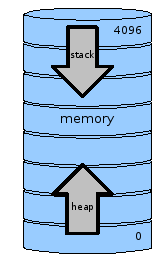
\includegraphics{images/instruction_memory.png}
	\end{center}
	\caption{instruction memory}
	\label{vm:instruction_memory:example}
\end{figure}
\section{Virtual machine instructions}
The vm offers serveral instructions to simulate a hardware cpu. As mentioned
before these instructions are based on the recommendation in \cite{wirth}
\\
The vm needs the instructions to be in a special format, the so-called
opCode-format, to be able to parse and execute them. The instructions are
divided into 3 groups depending on their opCode-format.
\\
\subsection{OpCode format 1}
The first format starts with an instruction-code (6 bit), followed by two 5 bit
and one 16 bit value. \\
\begin{tabular}{| p{1.5cm} | p{1.25cm} | p{1.25cm} | p{4cm} |}
			\hline
			(6 bit) & a(5 bit) & b(5 bit) & c(16 bit) \\ 
			\hline  
\end{tabular}
\\ \\
The following instructions are coded in this format: \\
ADDI, SUBI, MULI, DIVI, MODI, CMPI, CHKI, ANDI, BICI, ORI, XORI,
LSHI, ASHI, LDW, LDB, POP, STW, STB, PSH, BEQ, BNE, BLT, BGE, BGT, BLE
\\

\subsection{OpCode format 2}

The second format starts again with the 6 bit instruction-code, followed by 3 5
bit values. \\
\begin{tabular}{| p{1.5cm} | p{1.25cm} | p{1.25cm} | p{2.75cm} | p{1,25cm} |}
			\hline
			(6 bit) & a(5 bit) & b(5 bit) & 11 bit & c(5 bit) \\ 
			\hline  
\end{tabular}
\\ \\
ADD, SUB, MUL, DIV, MOD, CMP, CHK, AND, BIC, OR, XOR, LSH, ASH, PRNI, PRNC, PRNB

\subsection{OpCode format 3}
The third format contains the 6 bit instruction code, followed by a 16 bit
value. \\
\begin{tabular}{| p{1.5cm} | p{6.5cm} |}
			\hline
			(6 bit) & a(26 bit) \\ 
			\hline  
\end{tabular}
\\ \\
BSR, RET
\\ \\
All the mentioned instructions are taken from \cite{wirth}
except for the following:
\begin{description}
\item[PRNI] prints the integer value in register c to the console
\item[PRNC] prints the character value in register c to the console
\item[PRNB] prints the boolean value in register c to the console
\end{description}
The BSR instruction is expanded with a certain feature. If the value a is (-1)
the vm stops executing. \emph{BSR -1} is the so-called \emph{exit instruction}. 
